%%%%%%%%%%%%%%
%% Run LaTeX on this file several times to get Table of Contents,
%% cross-references, and citations.

%% If you have font problems, you may edit the w-bookps.sty file
%% to customize the font names to match those on your system.

%% w-bksamp.tex. Current Version: Feb 16, 2012
%%%%%%%%%%%%%%%%%%%%%%%%%%%%%%%%%%%%%%%%%%%%%%%%%%%%%%%%%%%%%%%%
%
%  Sample file for
%  Wiley Book Style, Design No.: SD 001B, 7x10
%  Wiley Book Style, Design No.: SD 004B, 6x9
%
%
%  Prepared by Amy Hendrickson, TeXnology Inc.
%  http://www.texnology.com
%%%%%%%%%%%%%%%%%%%%%%%%%%%%%%%%%%%%%%%%%%%%%%%%%%%%%%%%%%%%%%%%

%%%%%%%%%%%%%
% 7x10
%\documentclass{wileySev}

% 6x9
\documentclass{wileySix}

\usepackage{graphicx}
\usepackage{listings}

\usepackage{color}

\definecolor{codegreen}{rgb}{0,0.6,0}
\definecolor{codegray}{rgb}{0.5,0.5,0.5}
\definecolor{codepurple}{rgb}{0.58,0,0.82}
\definecolor{backcolour}{rgb}{0.95,0.95,0.92}

\lstdefinestyle{mystyle}{
    backgroundcolor=\color{backcolour},
    commentstyle=\color{codegreen},
    keywordstyle=\color{magenta},
    numberstyle=\tiny\color{codegray},
    stringstyle=\color{codepurple},
    basicstyle=\footnotesize,
    breakatwhitespace=false,
    breaklines=true,
    captionpos=b,
    keepspaces=true,
    numbers=left,
    numbersep=5pt,
    showspaces=false,
    showstringspaces=false,
    showtabs=false,
    tabsize=2,
    language=sh
}

\lstset{style=mystyle}

%%%%%%%
%% for times math: However, this package disables bold math (!)
%% \mathbf{x} will still work, but you will not have bold math
%% in section heads or chapter titles. If you don't use math
%% in those environments, mathptmx might be a good choice.

% \usepackage{mathptmx}

% For PostScript text
\usepackage{w-bookps}

%%%%%%%%%%%%%%%%%%%%%%%%%%%%%%%%%%%%%%%%%%%%%%%%%%%%%%%%%%%%%%%%
%% Other packages you might want to use:

% for chapter bibliography made with BibTeX
% \usepackage{chapterbib}

% for multiple indices
% \usepackage{multind}

% for answers to problems
% \usepackage{answers}

%%%%%%%%%%%%%%%%%%%%%%%%%%%%%%
%% Change options here if you want:
%%
%% How many levels of section head would you like numbered?
%% 0= no section numbers, 1= section, 2= subsection, 3= subsubsection
%%==>>
\setcounter{secnumdepth}{3}

%% How many levels of section head would you like to appear in the
%% Table of Contents?
%% 0= chapter titles, 1= section titles, 2= subsection titles,
%% 3= subsubsection titles.
%%==>>
\setcounter{tocdepth}{2}

%% Cropmarks? good for final page makeup
%% \docropmarks

%%%%%%%%%%%%%%%%%%%%%%%%%%%%%%
%
% DRAFT
%
% Uncomment to get double spacing between lines, current date and time
% printed at bottom of page.
% \draft
% (If you want to keep tables from becoming double spaced also uncomment
% this):
% \renewcommand{\arraystretch}{0.6}
%%%%%%%%%%%%%%%%%%%%%%%%%%%%%%

%%%%%%% Demo of section head containing sample macro:
%% To get a macro to expand correctly in a section head, with upper and
%% lower case math, put the definition and set the box
%% before \begin{document}, so that when it appears in the
%% table of contents it will also work:

\newcommand{\VT}[1]{\ensuremath{{V_{T#1}}}}

%% use a box to expand the macro before we put it into the section head:

\newbox\sectsavebox
\setbox\sectsavebox=\hbox{\boldmath\VT{xyz}}

%%%%%%%%%%%%%%%%% End Demo


\begin{document}


\booktitle{Cerdas Menguasai Python}
\subtitle{Dalam 24 Jam}

\authors{Rolly M. Awangga\\
\affil{Informatics Research Center}
%Floyd J. Fowler, Jr.\\
%\affil{University of New Mexico}
}

\offprintinfo{Cerdas Menguasai Python, First Edition}{Rolly M. Awangga}

%% Can use \\ if title, and edition are too wide, ie,
%% \offprintinfo{Survey Methodology,\\ Second Edition}{Robert M. Groves}

%%%%%%%%%%%%%%%%%%%%%%%%%%%%%%
%%
\halftitlepage

%\titlepage


\begin{copyrightpage}{2019}
%Survey Methodology / Robert M. Groves . . . [et al.].
%\       p. cm.---(Wiley series in survey methodology)
%\    ``Wiley-Interscience."
%\    Includes bibliographical references and index.
%\    ISBN 0-471-48348-6 (pbk.)
%\    1. Surveys---Methodology.  2. Social 
%\  sciences---Research---Statistical methods.  I. Groves, Robert M.  II. %
%Series.\\
%
%HA31.2.S873 2007
%001.4'33---dc22                                             2004044064
\end{copyrightpage}

\dedication{`Jika Kamu tidak dapat menahan lelahnya belajar,
Maka kamu harus sanggup menahan perihnya Kebodohan.'
~Imam Syafi'i~}

\begin{contributors}
\name{Rolly Maulana Awangga,} Informatics Research Center., Politeknik Pos Indonesia, Bandung,
Indonesia



\end{contributors}

\contentsinbrief
\tableofcontents
\listoffigures
\listoftables
\lstlistoflistings


\begin{foreword}
Sepatah kata dari Kaprodi, Kabag Kemahasiswaan dan Mahasiswa
\end{foreword}

\begin{preface}
Buku ini diciptakan bagi yang awam dengan flask sekalipun.

\prefaceauthor{R. M. Awangga}
\where{Bandung, Jawa Barat\\
Februari, 2019}
\end{preface}


\begin{acknowledgments}
Terima kasih atas semua masukan dari para mahasiswa agar bisa membuat buku ini 
lebih baik dan lebih mudah dimengerti.

Terima kasih ini juga ditujukan khusus untuk team IRC yang 
telah fokus untuk belajar dan memahami bagaimana buku ini mendampingi proses 
Intership.
\authorinitials{R. M. A.}
\end{acknowledgments}

\begin{acronyms}
\acro{ACGIH}{American Conference of Governmental Industrial Hygienists}
\acro{AEC}{Atomic Energy Commission}
\acro{OSHA}{Occupational Health and Safety Commission}
\acro{SAMA}{Scientific Apparatus Makers Association}
\end{acronyms}

\begin{glossary}
\term{git}Merupakan manajemen sumber kode yang dibuat oleh linus torvald.

\term{bash}Merupakan bahasa sistem operasi berbasiskan *NIX.

\term{linux}Sistem operasi berbasis sumber kode terbuka yang dibuat oleh Linus Torvald
\end{glossary}

\begin{symbols}
\term{A}Amplitude

\term{\hbox{\&}}Propositional logic symbol 

\term{a}Filter Coefficient

\bigskip

\term{\mathcal{B}}Number of Beats
\end{symbols}

\begin{introduction}

%% optional, but if you want to list author:

\introauthor{Rolly Maulana Awangga, S.T., M.T.}
{Informatics Research Center\\
Bandung, Jawa Barat, Indonesia}

Pada era disruptif  \index{disruptif}\index{disruptif!modern} 
saat ini. git merupakan sebuah kebutuhan dalam sebuah organisasi pengembangan perangkat lunak.
Buku ini diharapkan bisa menjadi penghantar para programmer, analis, IT Operation dan Project Manajer.
Dalam melakukan implementasi git pada diri dan organisasinya.

Rumusnya cuman sebagai contoh aja biar keren\cite{awangga2018sampeu}.

\begin{equation}
ABC {\cal DEF} \alpha\beta\Gamma\Delta\sum^{abc}_{def}
\end{equation}

\end{introduction}

%%%%%%%%%%%%%%%%%%Isi Buku_
%TEORI
%\chapter{Judul Bagian Pertama}
%\section{Arjun Yuda Firwanda}
\subsection{Soal 1}
Isi jawaban soal ke-1

Kalau mau dibikin paragrap \textbf{cukup enter aja}, tidak usah pakai \verb|par| dsb

%\subsection{Soal 2}
%Isi jawaban soal ke-2

%\subsection{Soal 3}
%Isi jawaban soal ke-3

\section{Dwi Yulianingsih}
\subsection{Soal 1}
Isi jawaban soal ke-1

Kalau mau dibikin paragrap \textbf{cukup enter aja}, tidak usah pakai \verb|par| dsb

%\subsection{Soal 2}
%Isi jawaban soal ke-2

%\subsection{Soal 3}
%Isi jawaban soal ke-3

\section{Harun Ar-Rasyid}
\subsection{Soal 1}
Isi jawaban soal ke-1

Kalau mau dibikin paragrap \textbf{cukup enter aja}, tidak usah pakai \verb|par| dsb

%\subsection{Soal 2}
%Isi jawaban soal ke-2

%\subsection{Soal 3}
%Isi jawaban soal ke-3

\section{Sri Rahayu}
\subsection{Soal 1}
Isi jawaban soal ke-1

Kalau mau dibikin paragrap \textbf{cukup enter aja}, tidak usah pakai \verb|par| dsb

%\subsection{Soal 2}
%Isi jawaban soal ke-2

%\subsection{Soal 3}
%Isi jawaban soal ke-3

\section{Doli Jonviter}
\subsection{Soal 1}
Isi jawaban soal ke-1

Kalau mau dibikin paragrap \textbf{cukup enter aja}, tidak usah pakai \verb|par| dsb

%\subsection{Soal 2}
%Isi jawaban soal ke-2

%\subsection{Soal 3}
%Isi jawaban soal ke-3

\section{Rahmatul Ridha}
\subsection{Soal 1}
Isi jawaban soal ke-1

Kalau mau dibikin paragrap \textbf{cukup enter aja}, tidak usah pakai \verb|par| dsb

%\subsection{Soal 2}
%Isi jawaban soal ke-2

%\subsection{Soal 3}
%Isi jawaban soal ke-3

\section{Tomy Prawoto}
\subsection{Soal 1}
Isi jawaban soal ke-1

Kalau mau dibikin paragrap \textbf{cukup enter aja}, tidak usah pakai \verb|par| dsb

%\subsection{Soal 2}
%Isi jawaban soal ke-2

%\subsection{Soal 3}
%Isi jawaban soal ke-3

%PRAKTEK
%\chapter{Judul Bagian Pertama}
%\section{Arjun Yuda Firwanda}
\subsection{Soal 1}
Isi jawaban soal ke-1

Kalau mau dibikin paragrap \textbf{cukup enter aja}, tidak usah pakai \verb|par| dsb

%\subsection{Soal 2}
%Isi jawaban soal ke-2

%\subsection{Soal 3}
%Isi jawaban soal ke-3

\section{Dwi Yulianingsih}
\subsection{Soal 1}
Isi jawaban soal ke-1

Kalau mau dibikin paragrap \textbf{cukup enter aja}, tidak usah pakai \verb|par| dsb

%\subsection{Soal 2}
%Isi jawaban soal ke-2

%\subsection{Soal 3}
%Isi jawaban soal ke-3

\section{Harun Ar-Rasyid}
\subsection{Soal 1}
Isi jawaban soal ke-1

Kalau mau dibikin paragrap \textbf{cukup enter aja}, tidak usah pakai \verb|par| dsb

%\subsection{Soal 2}
%Isi jawaban soal ke-2

%\subsection{Soal 3}
%Isi jawaban soal ke-3

\section{Sri Rahayu}
\subsection{Soal 1}
Isi jawaban soal ke-1

Kalau mau dibikin paragrap \textbf{cukup enter aja}, tidak usah pakai \verb|par| dsb

%\subsection{Soal 2}
%Isi jawaban soal ke-2

%\subsection{Soal 3}
%Isi jawaban soal ke-3

\section{Doli Jonviter}
\subsection{Soal 1}
Isi jawaban soal ke-1

Kalau mau dibikin paragrap \textbf{cukup enter aja}, tidak usah pakai \verb|par| dsb

%\subsection{Soal 2}
%Isi jawaban soal ke-2

%\subsection{Soal 3}
%Isi jawaban soal ke-3

\section{Rahmatul Ridha}
\subsection{Soal 1}
Isi jawaban soal ke-1

Kalau mau dibikin paragrap \textbf{cukup enter aja}, tidak usah pakai \verb|par| dsb

%\subsection{Soal 2}
%Isi jawaban soal ke-2

%\subsection{Soal 3}
%Isi jawaban soal ke-3

\section{Tomy Prawoto}
\subsection{Soal 1}
Isi jawaban soal ke-1

Kalau mau dibikin paragrap \textbf{cukup enter aja}, tidak usah pakai \verb|par| dsb

%\subsection{Soal 2}
%Isi jawaban soal ke-2

%\subsection{Soal 3}
%Isi jawaban soal ke-3


%TEORI
%\chapter{Judul Bagian Pertama}
%\section{Arjun Yuda Firwanda}
\subsection{Soal 1}
Isi jawaban soal ke-1

Kalau mau dibikin paragrap \textbf{cukup enter aja}, tidak usah pakai \verb|par| dsb

%\subsection{Soal 2}
%Isi jawaban soal ke-2

%\subsection{Soal 3}
%Isi jawaban soal ke-3

\section{Dwi Yulianingsih}
\subsection{Soal 1}
Isi jawaban soal ke-1

Kalau mau dibikin paragrap \textbf{cukup enter aja}, tidak usah pakai \verb|par| dsb

%\subsection{Soal 2}
%Isi jawaban soal ke-2

%\subsection{Soal 3}
%Isi jawaban soal ke-3

\section{Harun Ar-Rasyid}
\subsection{Soal 1}
Isi jawaban soal ke-1

Kalau mau dibikin paragrap \textbf{cukup enter aja}, tidak usah pakai \verb|par| dsb

%\subsection{Soal 2}
%Isi jawaban soal ke-2

%\subsection{Soal 3}
%Isi jawaban soal ke-3

\section{Sri Rahayu}
\subsection{Soal 1}
Isi jawaban soal ke-1

Kalau mau dibikin paragrap \textbf{cukup enter aja}, tidak usah pakai \verb|par| dsb

%\subsection{Soal 2}
%Isi jawaban soal ke-2

%\subsection{Soal 3}
%Isi jawaban soal ke-3

\section{Doli Jonviter}
\subsection{Soal 1}
Isi jawaban soal ke-1

Kalau mau dibikin paragrap \textbf{cukup enter aja}, tidak usah pakai \verb|par| dsb

%\subsection{Soal 2}
%Isi jawaban soal ke-2

%\subsection{Soal 3}
%Isi jawaban soal ke-3

\section{Rahmatul Ridha}
\subsection{Soal 1}
Isi jawaban soal ke-1

Kalau mau dibikin paragrap \textbf{cukup enter aja}, tidak usah pakai \verb|par| dsb

%\subsection{Soal 2}
%Isi jawaban soal ke-2

%\subsection{Soal 3}
%Isi jawaban soal ke-3

\section{Tomy Prawoto}
\subsection{Soal 1}
Isi jawaban soal ke-1

Kalau mau dibikin paragrap \textbf{cukup enter aja}, tidak usah pakai \verb|par| dsb

%\subsection{Soal 2}
%Isi jawaban soal ke-2

%\subsection{Soal 3}
%Isi jawaban soal ke-3

%PRAKTEK
%\chapter{Judul Bagian Pertama}
%\section{Arjun Yuda Firwanda}
\subsection{Soal 1}
Isi jawaban soal ke-1

Kalau mau dibikin paragrap \textbf{cukup enter aja}, tidak usah pakai \verb|par| dsb

%\subsection{Soal 2}
%Isi jawaban soal ke-2

%\subsection{Soal 3}
%Isi jawaban soal ke-3

\section{Dwi Yulianingsih}
\subsection{Soal 1}
Isi jawaban soal ke-1

Kalau mau dibikin paragrap \textbf{cukup enter aja}, tidak usah pakai \verb|par| dsb

%\subsection{Soal 2}
%Isi jawaban soal ke-2

%\subsection{Soal 3}
%Isi jawaban soal ke-3

\section{Harun Ar-Rasyid}
\subsection{Soal 1}
Isi jawaban soal ke-1

Kalau mau dibikin paragrap \textbf{cukup enter aja}, tidak usah pakai \verb|par| dsb

%\subsection{Soal 2}
%Isi jawaban soal ke-2

%\subsection{Soal 3}
%Isi jawaban soal ke-3

\section{Sri Rahayu}
\subsection{Soal 1}
Isi jawaban soal ke-1

Kalau mau dibikin paragrap \textbf{cukup enter aja}, tidak usah pakai \verb|par| dsb

%\subsection{Soal 2}
%Isi jawaban soal ke-2

%\subsection{Soal 3}
%Isi jawaban soal ke-3

\section{Doli Jonviter}
\subsection{Soal 1}
Isi jawaban soal ke-1

Kalau mau dibikin paragrap \textbf{cukup enter aja}, tidak usah pakai \verb|par| dsb

%\subsection{Soal 2}
%Isi jawaban soal ke-2

%\subsection{Soal 3}
%Isi jawaban soal ke-3

\section{Rahmatul Ridha}
\subsection{Soal 1}
Isi jawaban soal ke-1

Kalau mau dibikin paragrap \textbf{cukup enter aja}, tidak usah pakai \verb|par| dsb

%\subsection{Soal 2}
%Isi jawaban soal ke-2

%\subsection{Soal 3}
%Isi jawaban soal ke-3

\section{Tomy Prawoto}
\subsection{Soal 1}
Isi jawaban soal ke-1

Kalau mau dibikin paragrap \textbf{cukup enter aja}, tidak usah pakai \verb|par| dsb

%\subsection{Soal 2}
%Isi jawaban soal ke-2

%\subsection{Soal 3}
%Isi jawaban soal ke-3


%TEORI
%\chapter{Judul Bagian Pertama}
%\section{Arjun Yuda Firwanda}
\subsection{Soal 1}
Isi jawaban soal ke-1

Kalau mau dibikin paragrap \textbf{cukup enter aja}, tidak usah pakai \verb|par| dsb

%\subsection{Soal 2}
%Isi jawaban soal ke-2

%\subsection{Soal 3}
%Isi jawaban soal ke-3

\section{Dwi Yulianingsih}
\subsection{Soal 1}
Isi jawaban soal ke-1

Kalau mau dibikin paragrap \textbf{cukup enter aja}, tidak usah pakai \verb|par| dsb

%\subsection{Soal 2}
%Isi jawaban soal ke-2

%\subsection{Soal 3}
%Isi jawaban soal ke-3

\section{Harun Ar-Rasyid}
\subsection{Soal 1}
Isi jawaban soal ke-1

Kalau mau dibikin paragrap \textbf{cukup enter aja}, tidak usah pakai \verb|par| dsb

%\subsection{Soal 2}
%Isi jawaban soal ke-2

%\subsection{Soal 3}
%Isi jawaban soal ke-3

\section{Sri Rahayu}
\subsection{Soal 1}
Isi jawaban soal ke-1

Kalau mau dibikin paragrap \textbf{cukup enter aja}, tidak usah pakai \verb|par| dsb

%\subsection{Soal 2}
%Isi jawaban soal ke-2

%\subsection{Soal 3}
%Isi jawaban soal ke-3

\section{Doli Jonviter}
\subsection{Soal 1}
Isi jawaban soal ke-1

Kalau mau dibikin paragrap \textbf{cukup enter aja}, tidak usah pakai \verb|par| dsb

%\subsection{Soal 2}
%Isi jawaban soal ke-2

%\subsection{Soal 3}
%Isi jawaban soal ke-3

\section{Rahmatul Ridha}
\subsection{Soal 1}
Isi jawaban soal ke-1

Kalau mau dibikin paragrap \textbf{cukup enter aja}, tidak usah pakai \verb|par| dsb

%\subsection{Soal 2}
%Isi jawaban soal ke-2

%\subsection{Soal 3}
%Isi jawaban soal ke-3

\section{Tomy Prawoto}
\subsection{Soal 1}
Isi jawaban soal ke-1

Kalau mau dibikin paragrap \textbf{cukup enter aja}, tidak usah pakai \verb|par| dsb

%\subsection{Soal 2}
%Isi jawaban soal ke-2

%\subsection{Soal 3}
%Isi jawaban soal ke-3

%PRAKTEK
%\chapter{Judul Bagian Pertama}
%\section{Arjun Yuda Firwanda}
\subsection{Soal 1}
Isi jawaban soal ke-1

Kalau mau dibikin paragrap \textbf{cukup enter aja}, tidak usah pakai \verb|par| dsb

%\subsection{Soal 2}
%Isi jawaban soal ke-2

%\subsection{Soal 3}
%Isi jawaban soal ke-3

\section{Dwi Yulianingsih}
\subsection{Soal 1}
Isi jawaban soal ke-1

Kalau mau dibikin paragrap \textbf{cukup enter aja}, tidak usah pakai \verb|par| dsb

%\subsection{Soal 2}
%Isi jawaban soal ke-2

%\subsection{Soal 3}
%Isi jawaban soal ke-3

\section{Harun Ar-Rasyid}
\subsection{Soal 1}
Isi jawaban soal ke-1

Kalau mau dibikin paragrap \textbf{cukup enter aja}, tidak usah pakai \verb|par| dsb

%\subsection{Soal 2}
%Isi jawaban soal ke-2

%\subsection{Soal 3}
%Isi jawaban soal ke-3

\section{Sri Rahayu}
\subsection{Soal 1}
Isi jawaban soal ke-1

Kalau mau dibikin paragrap \textbf{cukup enter aja}, tidak usah pakai \verb|par| dsb

%\subsection{Soal 2}
%Isi jawaban soal ke-2

%\subsection{Soal 3}
%Isi jawaban soal ke-3

\section{Doli Jonviter}
\subsection{Soal 1}
Isi jawaban soal ke-1

Kalau mau dibikin paragrap \textbf{cukup enter aja}, tidak usah pakai \verb|par| dsb

%\subsection{Soal 2}
%Isi jawaban soal ke-2

%\subsection{Soal 3}
%Isi jawaban soal ke-3

\section{Rahmatul Ridha}
\subsection{Soal 1}
Isi jawaban soal ke-1

Kalau mau dibikin paragrap \textbf{cukup enter aja}, tidak usah pakai \verb|par| dsb

%\subsection{Soal 2}
%Isi jawaban soal ke-2

%\subsection{Soal 3}
%Isi jawaban soal ke-3

\section{Tomy Prawoto}
\subsection{Soal 1}
Isi jawaban soal ke-1

Kalau mau dibikin paragrap \textbf{cukup enter aja}, tidak usah pakai \verb|par| dsb

%\subsection{Soal 2}
%Isi jawaban soal ke-2

%\subsection{Soal 3}
%Isi jawaban soal ke-3


%TEORI
\chapter{Library CSV dan Pandas}
\section{Luthfi Muhammad Nabil/1174035}
\subsection{Soal 1}
Fungsi, Sejarah, dan Contoh file CSV : 
\begin{itemize}
	\item Fungsi : 
	File CSV (Comma Separated Values) adalah tipe file khusus yang menyimpan informasi dengan metode dipisahkan dengan koma. File CSV berfungsi untuk menjadi perantara untuk beberapa aplikasi yang memiliki basis data saat mengirim data. CSV dapat dibuka di berbagai text editor
	yang ada. Dengan bentuk filenya yang dinamis memungkinkan file CSV dapat dimanipulasi dan dapat menyimpan informasi dengan skala besar.
	\item Sejarah :
	CSV sudah digunakan sejak tahun 1972 yang dapat dikompilasi pada bahasa pemrograman IBM Fortran. Saat itu, data yang dipisahkan oleh koma jika isinya memiliki spasi maka harus diberi tanda petik di awal dan akhir isi dari data tersebut. Nama CSV baru mulai digunakan pada tahun 1983. Pada panduan dari Osborne Executive Computer mendokumentasikan kutipan yang membolehkan isi karakter memiliki koma.  Pada tahun 2005 dengan RFC4180, CSV didefinisikan sebagai MIME Content Type. lalu pada tahun 2013, defisiensi dari RFC4180 dipecahkan oleh rekomendasi dari W3C. Pada tahun 2014, IETF mempublikasi RFC7111 yang mendeskripsikan pecahan Uniform Resource Identifier(URI) ke dokumen CSV. RFC7111 menjelaskan bagaimana baris, kolom dapat dipilih dalam dokumen CSV menggunakan indeks posisi. Pada Tahun 2015, W3C mempublikasikan draft rekomendasi untuk CSV-metadata standards yang dimulai dengan rekomendasi pada bulan Desember dengan tahun yang sama. 
	\item Contoh File CSV \begin{itemize}
							\item 
							CSV pada Excel \ref{1174035_CSVExcel}
							\begin{figure}[!htbp]
								\centering
								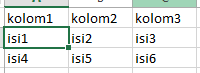
\includegraphics[height=4cm, width=7cm]{figures/4/1174035/Teori/1174035_CSVExcel.jpg}
								\caption{Contoh CSV Pada Excel}
								\label{1174035_CSVExcel}
							\end{figure}
							\item \begin{figure}[!htbp]
								\centering
								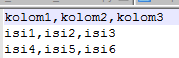
\includegraphics[height=4cm, width=7cm]{figures/4/1174035/Teori/1174035_CSVText.jpg}
								\caption{Contoh CSV Pada Text}
								\label{1174035_CSVText}
							\end{figure}
							CSV pada Text Editor \ref{1174035_CSVText}
							
						  \end{itemize}
\end{itemize}
\subsection{Soal 2}
Aplikasi Yang dapat membuat file CSV : 
Berikut file yang dapat membuat file CSV
\begin{itemize}
	\item Spreadsheet :
	Spreadsheet merupakan aplikasi yang dapat membuat CSV hanya dengan memasukan data sesuai baris dan kolom yang diinginkan. Contoh spreadsheet seperti Google Spreadsheet, Microsoft Excel, dan aplikasi lainnya. 
	\item Bahasa Pemrograman :
	Bahasa pemrograman merupakan media yang dapat untuk membuat aplikasi yang dapat membuat file CSV khusus untuk bahasa pemrograman yang support dengan pembuatan file CSV. Seperti Python, C Sharp, dan lain sebagainya.
	\item Text Editor :
	Text editor juga dapat membuat file CSV, untuk membuat dengan Text Editor cukup dengan membuat file sesuai format CSV dan save file tersebut dengan ekstensi .CSV.
\end{itemize}
\subsection{Soal 3}
Menulis dan Membaca file CSV : 
Berikut cara menulis dan membaca file CSV : 
\begin{itemize}
	\item Menulis : \begin{enumerate}
						\item Buka file CSV dengan spreadsheet
						\item Klik Cell yang mau diisi
						\item Masukan data yang mau diisi pada cell tersebut
						\item Lalu save file dengan format .CSV
					\end{enumerate}
	\item Membaca : \begin{enumerate}
						\item Buka file CSV dengan spreadsheet						
					\end{enumerate}
\end{itemize}
\subsection{Soal 4}
Sejarah Library CSV Python : 
Library CSV pada python merupakan library yang paling umum untuk import export data pada spreadsheet dan basis data dengan format sesuai dengan standarisasi RFC4180. Seiring dengan lahirnya bahasa pemrograman python, library mulai dibuat dan dikembangkan sampai akhirnya pada tahun 2003, pembuatnya Kevin Altis dan lainnya telah merilis versi final untuk library Python CSV. 
\subsection{Soal 5}
Sejarah Library Pandas Python : 
Pandas (Python Data Analysis Library) adalah library open source yang digunakan untuk melakukan data manajemen dan data analysis. Pandas diciptakan pada tahun 2008 oleh Wes McKinney dan diperbaharui oleh Sien Chang pada tahun 2010. Inspirasi dari pembuatan pandas muncul pada komunitas yang membutuhkan library khusus untuk analisis data. 
\subsection{Soal 6}
Fungsi - fungsi yang terdapat di library CSV : 
\begin{itemize}
	\item \begin{verbatim} csv.reader(csvfile, dialect='excel', **fmtparams) \end{verbatim} Untuk mengembalikan	object reader yang akan mengambil setiap line pada csv yang diambil. Data setiap baris diambil saat next() dipanggil. Berikut contohnya : \lstinputlisting[firstline=1, lastline=6]{src/4/1174035/Teori/chap4_1174035_teori.py}
	\item \begin{verbatim} csv.writer(csvfile, dialect='excel', **fmtparams) \end{verbatim} Mengembalikan file pembuat object untuk dapat mengkonversi data pada python ke file CSV yang akan dibuat. Berikut contoh penggunaan csv.writer : \lstinputlisting[firstline=8, lastline=14]{src/4/1174035/Teori/chap4_1174035_teori.py}
	\item \begin{verbatim} csv.register_dialect(name[, dialect[, **fmtparams]]) \end{verbatim} Mengasosiasikan dialek dengan nama, nama yang dimasukkan harus berupa karakter.
	\item \begin{verbatim} csv.unregister_dialect(name) \end{verbatim}
	Menghapus asosiasi dialek dengan nama pada registry dialek.
	\item \begin{verbatim} csv.get_dialect(name) \end{verbatim}
	Mengambil dialek yang telah diasosiasikan dengan nama. 
	\item \begin{verbatim}  csv.list_dialects() \end{verbatim} Mengembalikan dialek yang telah diregistrasi.
	\item \begin{verbatim} csv.field_size_limit([new_limit]) \end{verbatim} Mengembalikan maksimal kolom data yang diperbolehkan oleh pembaca.
\end{itemize}
\subsection{Soal 7}
Fungsi - fungsi yang terdapat di library Pandas : 
\begin{itemize}
	\item \begin{verbatim} pandas.read_csv(filepath_or_buffer[, sep, …]) \end{verbatim} Untuk membaca file CSV dan menyimpannya ke DataFrame
	\item \begin{verbatim} pandas.read_excel(io[, sheet_name, header, names, …])  \end{verbatim} Membaca file excel dan menyimpannya ke DataFrame
	\item \begin{verbatim} to_csv([path, index, sep, na_rep, …]) \end{verbatim}
	Untuk membuat file CSV dari data yang ada	
\end{itemize}
\subsection{Cek Plagiarism}
Berikut pengecekan plagiarism yang dilakukan pada website smallseotools.com : 
\begin{figure}[!htbp]
	\centering
	\includegraphics[height=6cm, width=10cm]{figures/4/1174035/Teori/1174035_plagiarism.png}
	\caption{Cek Plagiarisme}
	\label{1174035_plagiarism}
\end{figure}

\section{Hagan Rowlenstino/1174040}
	\subsection{Soal 1}
	format file csv dapat menyimpan data dalam jumlah yang sangat besar juga diperuntukkan untuk export dan import untuk spreadsheet ataupun database. Singkatan CSV pertamakali di pakai pada tahun 1983, dimana value yang dipisahkan dengan koma lebih mudah untuk diketik daripada data yang sejajar dengan kolom yang tetap. contohnya seperti gambar dibawah ini.

	\begin{figure}[ht]
            \centerline{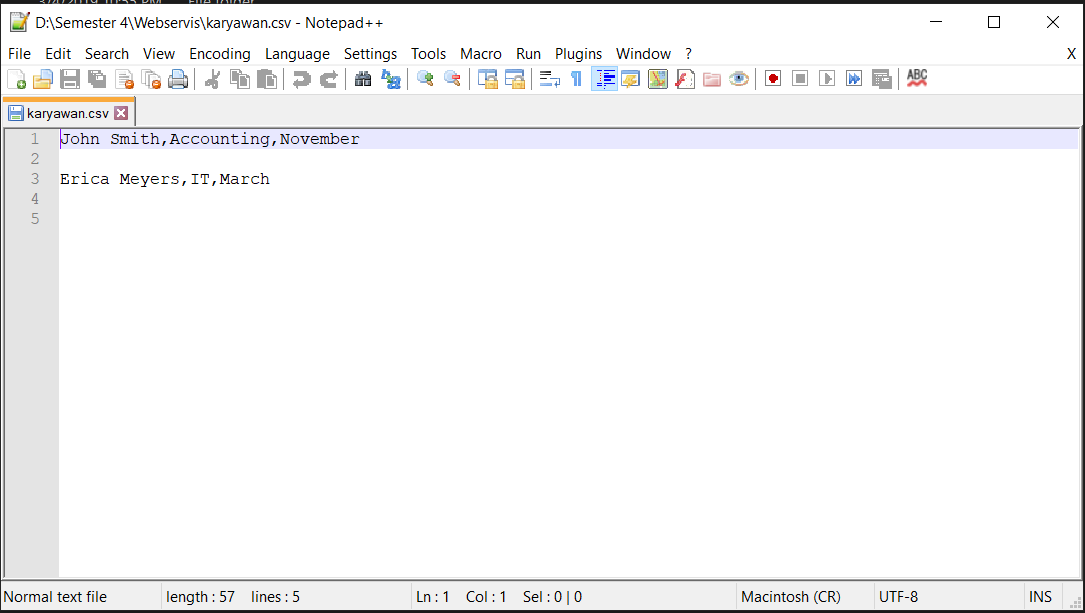
\includegraphics[width=0.5\textwidth]{figures/4/1174040/Teori/1174040_csv.png}}
            \caption{Contoh CSV}
            \label{1174040_csv}
            \end{figure}

    \subsection{Soal 2}
    Ms.Excel , NotePad, notepad++, sublime, dan texteditor lainnya

    \subsection{Soal 3}
    caranya adalah :
		\begin{itemize}
			\item untuk write :
			\begin{enumerate}
				\item Download template csv
				\item Buka browser lalu menuju ke Google Sheet
				\item Tekan tombol merah di pojok kanan bawah
				\item Lalu pilih upload file untuk mengupload template yang sudah di download sebelumya
				\item Edit sesuai yang diinginkan
				\item Setelah selesai, lalukan eksport ke CSV dengan cara klik file lalu download as setelah itu pilih CSV
			\end{enumerate}
			\item untuk read :
			\begin{enumerate}
				\item buka Ms.Excel
				\item pilih Data lalu Get External Data dan pilih From Text
				\item lalu pilih file csv nya
				\item pilih Delimeted lalu Next
				\item checklist di box Tab dan Comma
				\item lalu klik finish
			\end{enumerate}
		\end{itemize}

	\subsection{Soal 4}
	Library umum dalam CSV yang gunanya untuk import dan export data di dalam database yang terstandarisasi RFC4180 yang berisikan fungsi -fungsi dan kelas yang akan dipakai dalam pengerjaan file CSV.

	\subsection{Soal 5}
	Pandas diciptakan pada tahun 2008 oleh Wes McKinney dan diperbaharuin pada tahun 2010 oleh Sien Chang. yang fungsinya untuk melakukan analisa data seperti import dan export data.

	\subsection{Soal 6}
	Fungsi - funsi library csv adalah :
		\begin{itemize}
			
			\item \begin{verbatim}csv.reader(csvfile, dialect='excel', **fmtparams)\end{verbatim} : digunakan untuk membaca line di csv
			\item \begin{verbatim}csv.writer(csvfile, dialect='excel', **fmtparams)\end{verbatim} : untuk menulis line di csv
			\item \begin{verbatim}csv.register_dialect(name[, dialect[, **fmtparams]]) \end{verbatim}: untuk asosiasikan dialect dengan name, dimana name harus string
			\item \begin{verbatim}csv.unregister_dialect(name)\end{verbatim} : menghapus dialect yang terasosiasi dengan name
			\item \begin{verbatim}csv.get_dialect(name)\end{verbatim} : mengnembalikan hasil dialect yang terasosisasi dengan name
			\item \begin{verbatim}csv.list_dialects() \end{verbatim}: menampilkan semua dialect yang ada
			\item \begin{verbatim}csv.field_size_limit([new_limit])\end{verbatim} : menamplikan field maksimal ayng di berikan oleh pembubat parse.

		\end{itemize}

	\subsection{Soal 7}
	Fungsi - fungsi yang terdapat di library Pandas : 
\begin{itemize}
	\item \begin{verbatim} pandas.read_csv(filepath_or_buffer[, sep, …]) \end{verbatim} : Untuk membaca file CSV
	\item \begin{verbatim} pandas.read_excel(io[, sheet_name, header, names, …])  \end{verbatim} : Membaca file excel 
	\item \begin{verbatim} to_csv([path, index, sep, na_rep, …]) \end{verbatim} : Untuk me write ke dalam file csv	
\end{itemize}
	
	\subsection{Cek Plagiarisme}
	\begin{figure}[ht]
            \centerline{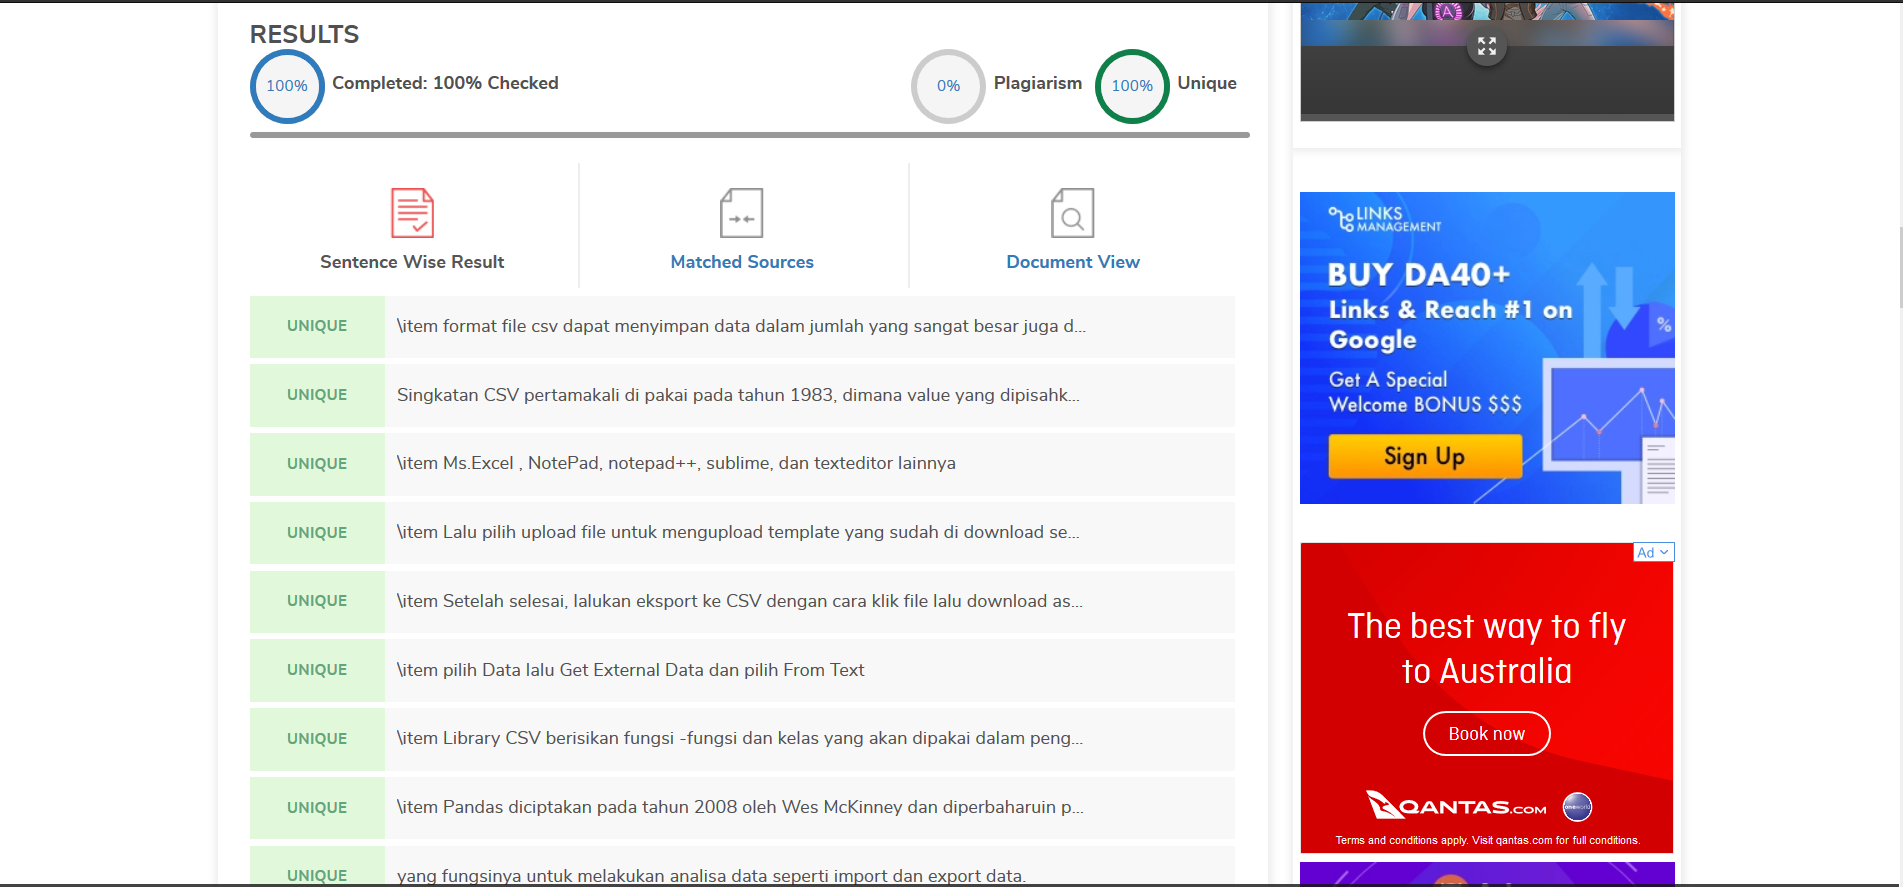
\includegraphics[width=0.5\textwidth]{figures/4/1174040/Teori/1174040_plagiat.png}}
            \caption{Plagiarisme}
            \label{1174040_plagiat}
            \end{figure}
			

\section{Faisal Najib Abdullah 1174042}
\subsection{Pemahaman Teori}
\begin{enumerate}
    \item Apa itu fungsi file csv, jelaskan sejarah dan contoh ?
    \par
    File CSV Nilai Berbatas Koma adalah tipe file khusus yang dapat Anda buat atau edit di Excel. File CSV menyimpan informasi yang dipisahkan oleh koma, bukan menyimpan informasi dalam kolom. Saat teks dan angka disimpan dalam file CSV, mudah untuk memindahkannya dari satu program ke program lain.
    \par 
	File CSV dibuat oleh program yang menangani sejumlah data yang besar. CSV merupakan cara yang nyaman untuk mengekspor data dari spreadsheet dan basis data serta mengimpor atau menggunakannya dalam program lain. Misalnya, Anda dapat mengekspor hasil program penambangan data ke file CSV dan kemudian mengimpornya ke dalam spreadsheet untuk menganalisis data, menghasilkan grafik untuk presentasi, atau menyiapkan laporan untuk publikasi.
    \par
	Contohnya, Anda dapat mengekspor kontak dari Google ke dalam file CSV, kemudian mengimpornya ke Outlook.
    
    \item Aplikasi-aplikasi apa saja yang bisa menciptakan file csv?
    Pada Windows
    \begin{itemize}
        \item Microsoft Excel 2013
        \item Microsoft Works
        \item CCorel Quattro Pro
        \item Apache OpenOffice
        \item LibreOffice
        \item Microsoft Notepad
        \item Intuit Quicken 2015
        \item GenScriber
    \end{itemize}
    Pada Mac OS
    \begin{itemize}
        \item Microsoft Excel 2011
        \item Planamesa NeoOffice
        \item Apache OpenOffice
        \item LibreOffice
        \item GenScriber
    \end{itemize}
    Pada Linux
    \begin{itemize}
        \item Apache OpenOffice
        \item LibreOffice
        \item GenScriber
    \end{itemize}
    
    \item Jelaskan bagaimana cara menulis dan membaca file csv di excel atau spreadsheet?
	\begin{itemize}
        \item Cara menulis file csv harus berupa baris dan kolom atau bisa juga di sebut berupa tabel.
        \item Untuk membacanya file csv dipisahkannya menggunakan koma atau titik koma.
    \end{itemize}
    
    \item Jelaskan sejarah library csv?
	Library csv menyediakan fungsionalitas untuk membaca dan menulis ke file CSV. Dirancang untuk bekerja di luar kotak dengan file CSV yang dihasilkan Excel, memudahkan untuk bekerja dengan berbagai format CSV. Library csv berisi objek dan kode lain untuk membaca, menulis, dan memproses data ke file CSV.
    
    \item Jelaskan sejarah library pandas?
	panda adalah pustaka Python open-source yang menyediakan alat analisis data kinerja tinggi dan struktur data yang mudah digunakan. panda tersedia untuk semua instalasi Python, tetapi itu adalah bagian penting dari distribusi Anaconda dan bekerja sangat baik di notebook Jupyter untuk berbagi data, kode, hasil analisis, visualisasi, dan teks naratif.

    \item Jelaskan fungsi-fungsi yang terdapat di library csv?
	Terdapat 2 fungsi yang bisa digunakan oleh library csv
    Pertama,fungsi membaca file csv.
    fungsi ini bisa menggunakan list dan dictionary
    Dengan list :
    \lstinputlisting[firstline=11, lastline=21]{src/4/1174042/Teori/1174042_csv.py}
    Dengan dictionary :
    \lstinputlisting[firstline=24, lastline=33]{src/4/1174042/Teori/1174042_csv.py}
    Kedua,fungsi menulis file csv.
    \lstinputlisting[firstline=36, lastline=40]{src/4/1174042/Teori/1174042_csv.py}
    
    \item Jelaskan fungsi-fungsi yang terdapat di library pandas
	Hampir sama dengan library csv,tp library pandas penulisannya lebih sederhana dan terlihat lebih rapih dari pada library csv.
    \lstinputlisting[firstline=43, lastline=44]{src/4/1174042/Teori/1174042_csv.py}
\end{enumerate}

\subsection{Cek Plagiarism}
Berikut pengecekan plagiarism yang dilakukan pada website smallseotools.com : 
\begin{figure}[!htbp]
	\centering
	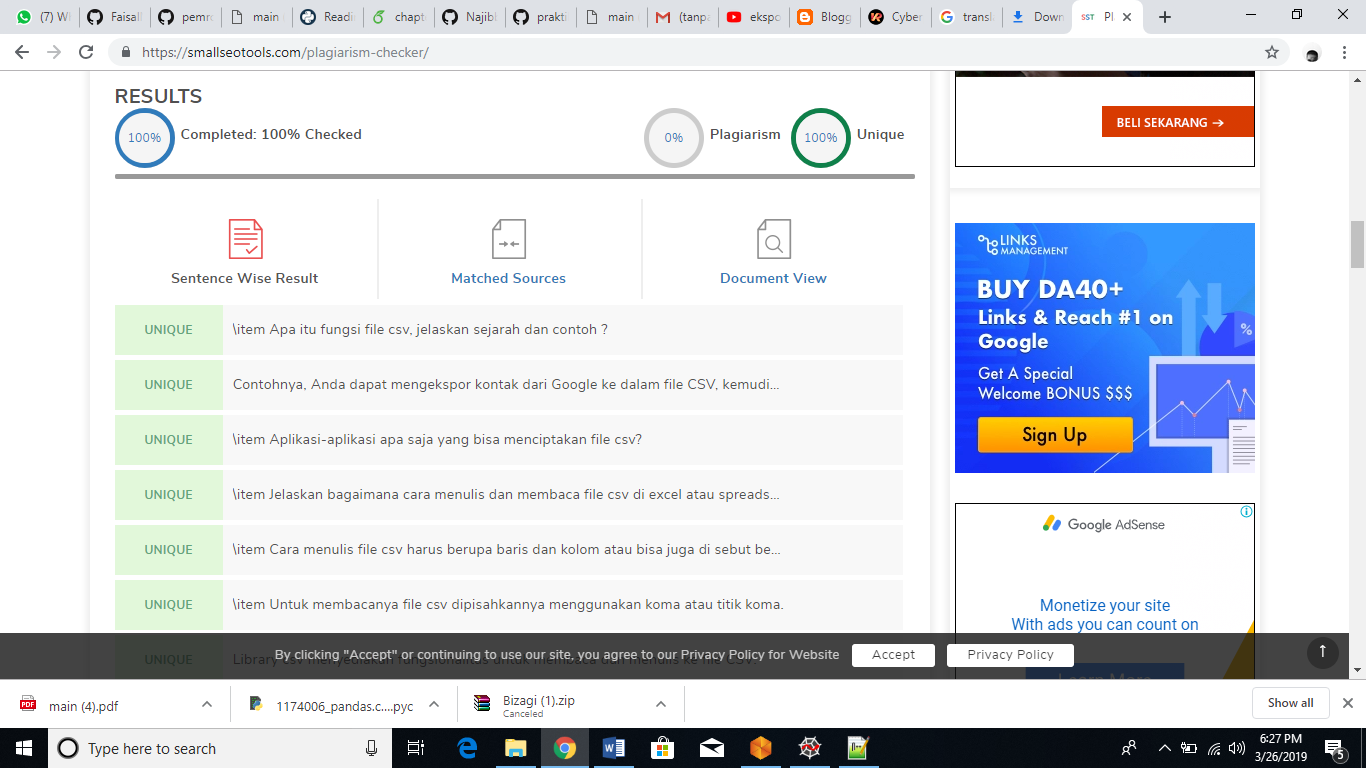
\includegraphics[height=6cm, width=10cm]{figures/4/1174042/1174042_plagiat.png}
	\caption{Cek Plagiarisme}
	\label{}
\end{figure}
%PRAKTEK
\chapter{Praktek Library CSV dan Pandas}
\section{Luthfi Muhammad Nabil/1174035}
\subsection{Soal 1}
Buatlah fungsi pada file chap4\_1174035\_csv.py untuk membuka file csv dengan lib csv mode list : 
\lstinputlisting[firstline=2, lastline=6]{src/4/1174035/Praktek/chap4_1174035_csv.py}

\subsection{Soal 2}
Buatlah fungsi pada file chap4\_1174035\_csv.py untuk membuka file csv dengan lib csv mode dictionary : 
\lstinputlisting[firstline=8, lastline=12]{src/4/1174035/Praktek/chap4_1174035_csv.py}

\subsection{Soal 3}
Buatlah fungsi pada file chap4\_1174035\_pandas.py untuk membuka file csv dengan lib pandas mode list : 
\lstinputlisting[firstline=2, lastline=5]{src/4/1174035/Praktek/chap4_1174035_pandas.py}

\subsection{Soal 4}
Buatlah fungsi pada file chap4\_1174035\_pandas.py untuk membuka file csv dengan lib pandas mode dictionary : 
\lstinputlisting[firstline=6, lastline=10]{src/4/1174035/Praktek/chap4_1174035_pandas.py}

\subsection{Soal 5}
Buatlah fungsi baru di chap4\_1174035\_pandas.py untuk mengubah format tanggal menjadi standard dataframe : 
\lstinputlisting[firstline=11, lastline=13]{src/4/1174035/Praktek/chap4_1174035_pandas.py}

\subsection{Soal 6}
Buatlah fungsi baru di chap4\_1174035\_pandas.py untuk mengubah index kolom : 
\lstinputlisting[firstline=14, lastline=16]{src/4/1174035/Praktek/chap4_1174035_pandas.py}

\subsection{Soal 7}
Buatlah fungsi baru di chap4\_1174035\_pandas.py untuk mengubah atribut atau nama kolom : 
\lstinputlisting[firstline=17, lastline=19]{src/4/1174035/Praktek/chap4_1174035_pandas.py}

\subsection{Soal 8}
Buatlah program chap4\_1174035\_main.py yang menggunakan library chap4\_1174035\_csv.py yang membuat dan membaca file CSV : 
\lstinputlisting{src/4/1174035/Praktek/chap4_1174035_main.py}

\subsection{Soal 9}
Buatlah program chap4\_1174035\_main2.py yang menggunakan library chap4\_1174035\_csv.py yang membuat dan membaca file CSV : 
\lstinputlisting{src/4/1174035/Praktek/chap4_1174035_main2.py}

\subsection{Penanganan Error}
Error yang didapat : KeyError
Deskripsi : Error saat kunci ada yang salah atau tidak ada di dalam file CSV 
\begin{figure}[!htbp]
	\centering
	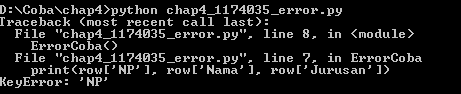
\includegraphics[height=4cm, width=10cm]{figures/4/1174035/Praktek/chap4_1174035_error.png}
	\caption{Contoh KeyError}
	\label{1174035_Error}
\end{figure}
Penanganan : Menggunakan KeyError seperti pada line berikut : \lstinputlisting{src/4/1174035/Praktek/chap4_1174035_error.py}
\begin{figure}[!htbp]
	\centering
	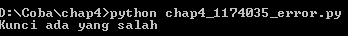
\includegraphics[height=4cm, width=10cm]{figures/4/1174035/Praktek/chap4_1174035_errorfix.png}
	\caption{Hasil Penanganan Error}
	\label{1174035_ErrorFix}
\end{figure}

\section{Hagan Rowlenstino/1174040}
\subsection{Soal 1}
Buatlah fungsi untuk membuka file csv dengan lib csv mode list : 
\lstinputlisting{src/4/1174040/Praktek/1174040_CSV1.py}

\subsection{Soal 2}
Buatlah fungsi untuk membuka file csv dengan lib csv mode dictionary : 
\lstinputlisting{src/4/1174040/Praktek/1174040_CSV2.py}

\subsection{Soal 3}
Buatlah fungsi  untuk membuka file csv dengan lib pandas mode list : 
\lstinputlisting{src/4/1174040/Praktek/1174040_pandas1.py}

\subsection{Soal 4}
Buatlah fungsi  untuk membuka file csv dengan lib pandas mode dictionary : 
\lstinputlisting{src/4/1174040/Praktek/1174040_pandas2.py}

\subsection{Soal 5}
Buatlah fungsi untuk mengubah format tanggal menjadi standard dataframe : 
\lstinputlisting{src/4/1174040/Praktek/1174040_pandas3.py}

\subsection{Soal 6}
Buatlah fungsi  untuk mengubah index kolom : 
\lstinputlisting{src/4/1174040/Praktek/1174040_pandas4.py}

\subsection{Soal 7}
Buatlah fungsi  untuk mengubah atribut atau nama kolom : 
\lstinputlisting{src/4/1174040/Praktek/1174040_pandas5.py}

\subsection{Soal 8}
Disini saya telah membuat file CSV bernama 1174040\_csv.csv untuk di tampilkan, dan sebelum me write ke dalam file csv, terlebih dahulu buat file 1174040\_writecsv.csv : 
\lstinputlisting{src/4/1174040/Praktek/1174040_main.py}

\subsection{Soal 9}
Disini saya telah membuat file CSV bernama 1174040\_csvpandas.csv untuk ditampilkan, dan sebelum me write ke dalam file csv, telebih dahulu buat file 1174040\_writepandas.csv : 
\lstinputlisting{src/4/1174040/Praktek/1174040_main2.py}

\bibliographystyle{IEEEtran}
%\def\bibfont{\normalsize}
\bibliography{references}


%%%%%%%%%%%%%%%
%%  The default LaTeX Index
%%  Don't need to add any commands before \begin{document}
\printindex

%%%% Making an index
%%
%% 1. Make index entries, don't leave any spaces so that they
%% will be sorted correctly.
%%
%% \index{term}
%% \index{term!subterm}
%% \index{term!subterm!subsubterm}
%%
%% 2. Run LaTeX several times to produce <filename>.idx
%%
%% 3. On command line, type  makeindx <filename> which
%% will produce <filename>.ind
%%
%% 4. Type \printindex to make the index appear in your book.
%%
%% 5. If you would like to edit <filename>.ind
%% you may do so. See docs.pdf for more information.
%%
%%%%%%%%%%%%%%%%%%%%%%%%%%%%%%

%%%%%%%%%%%%%% Making Multiple Indices %%%%%%%%%%%%%%%%
%% 1.
%% \usepackage{multind}
%% \makeindex{book}
%% \makeindex{authors}
%% \begin{document}
%%
%% 2.
%% % add index terms to your book, ie,
%% \index{book}{A term to go to the topic index}
%% \index{authors}{Put this author in the author index}
%%
%% \index{book}{Cows}
%% \index{book}{Cows!Jersey}
%% \index{book}{Cows!Jersey!Brown}
%%
%% \index{author}{Douglas Adams}
%% \index{author}{Boethius}
%% \index{author}{Mark Twain}
%%
%% 3. On command line type
%% makeindex topic
%% makeindex authors
%%
%% 4.
%% this is a Wiley command to make the indices print:
%% \multiprintindex{book}{Topic index}
%% \multiprintindex{authors}{Author index}

\end{document}

